\documentclass[12pt]{article}
%Gummi|065|=)
\usepackage{amsmath, amsfonts, amssymb}
\usepackage[margin=0.5in]{geometry}
\usepackage{xcolor}
\usepackage{graphicx}

\newcommand{\off}[1]{}
\DeclareMathSizes{20}{30}{20}{18}

\newcommand{\two }{\sqrt[3]{2}}
\newcommand{\four}{\sqrt[3]{4}}


\usepackage{tikz}

\title{Nilsequences}
\author{John D Mangual}
\date{}
\begin{document}

\fontfamily{qag}\selectfont \fontsize{12.5}{15}\selectfont

\maketitle

\noindent Terence Tao sees a lot of things, but he writes in an obfuscated way, and I think he misses a lot of things.  About 10 years ago, I was introduced to the topic of \textbf{nilsequences} in a course of Dynamics and Number Theory.  I did nothing with it.  Let's read Terry's latest blog on this topic\footnote{\texttt{https://terrytao.wordpress.com/2017/04/28/notes-on-nilcharacters-and-their-symbols/}}. \\ \\
Part of it is like\dots where do fractions come from?  \\ \\
If we take scientific measurement, there's quite a bit error that obstructs us from observing the most delicate patterns.  In fact, shielding us completely from finding them (or protecting us). \\ \\
$\sqrt{2} = 1.414213562373095048801688724209698078
5696718753769480731766797379907324784621070388503 $ \\ \\
If you examine the digits carefully\footnote{\texttt{http://www.gutenberg.org/files/129/129.txt}} we can prove the decimals do not exhibit any pattern in the decimal expension.  However, if we use continued fractions: \\ \\
$\sqrt{2} = [1; 2,2,2,2,2 , \dots ] $
and this is a nicer system since we have exponential convergence of the the number.  Here the error is $10^{-6}$ (microscopic). \\ \\
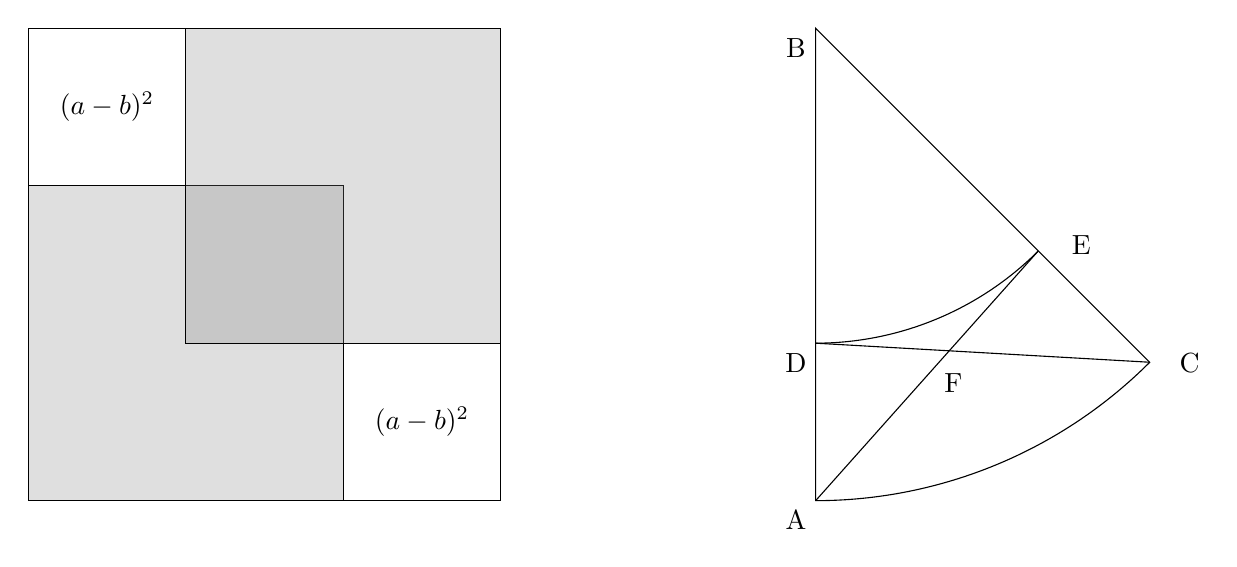
\begin{tikzpicture}

\begin{scope}
\draw (0,0)--(6,0)--(6,6)--(0,6)--cycle;
\draw[opacity=0.25, fill=black!50!white] (0,0)--(4,0)--(4,4)--(0,4)--cycle;
\draw (0,0)--(4,0)--(4,4)--(0,4)--cycle;
\draw[opacity=0.25, fill=black!50!white] (2,2)--(6,2)--(6,6)--(2,6)--cycle;
\draw (2,2)--(6,2)--(6,6)--(2,6)--cycle;
\node at (1,5) {$(a-b)^2$};
\node at (5,1) {$(a-b)^2$};
\end{scope}

\begin{scope}[xshift=10cm]

\draw (0,6)--(0,0)--(0,0) arc (90:135:-6)--cycle;
\draw (0,2) arc (90:135:-4);
\node at (-0.25,-0.25) {A};
\node at (-0.25,-0.25+6) {B};
\node at (-0.25+5,-0.25+2) {C};
\node at (-0.25,-0.25+2) {D};
\node at (-0.25+3.625,-0.25+3.5) {E};
\node at (-0.25+2,-0.25+1.75) {F};
\draw (0,2)--(6*1.414/2, 6 - 6*1.414/2);
\draw (0,0)--(4*1.414/2, 6 - 4*1.414/2);

\end{scope}

\end{tikzpicture} \\
These pictures lead to two different proofs that $\sqrt{2} \notin \mathbb{Q}$.  They are both geometric proofs, and argue by infinite descent.  Therefore, there must have been an \`{e}tale cohomology. \\ \\
I have no idea what \`{e}tale cohomology and the books do not simplify it enough for me. \\ 
Forget it.  One way to get meaningful numbers to arbitrary accuracy is to observe a dynamical system over time and take detailed measurements.  And you will see.

\newpage

\noindent Using a minimimal amount of math we can define most (possibly all) nilsequences.  The fractional part of multiples of $\sqrt{2}$ is nilsequence. \\

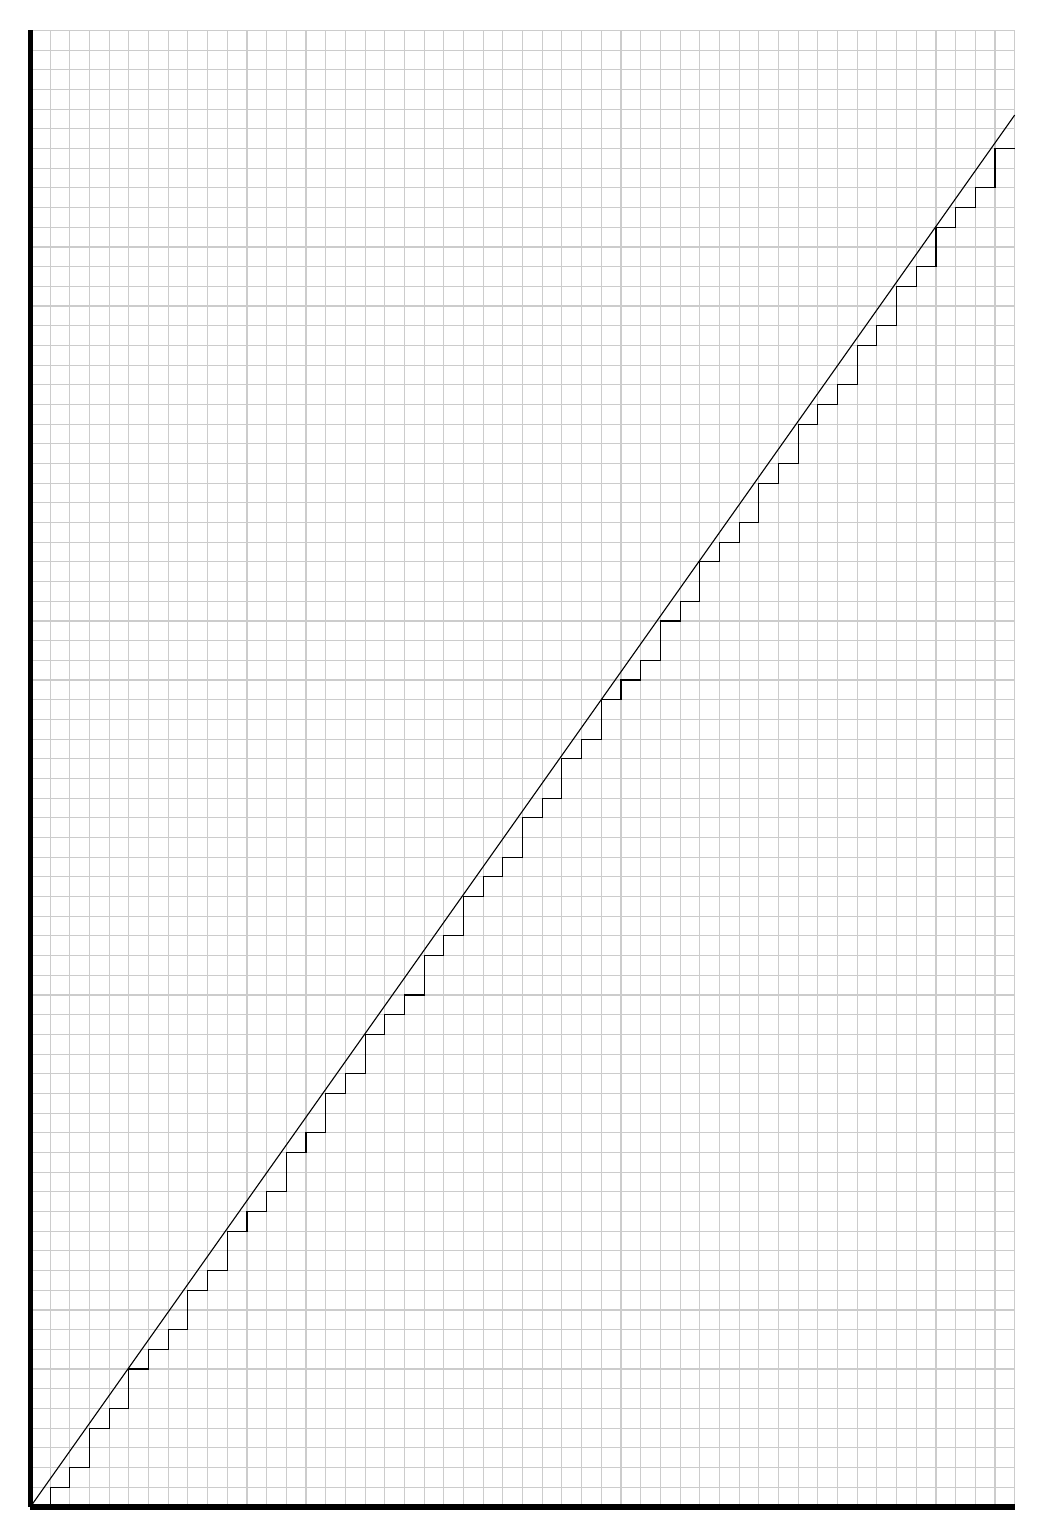
\begin{tikzpicture}[scale=0.25]

\foreach \a in {0,...,50}{
	\draw[color=black!20!white] (\a, 0)--(\a, 75);
}

\foreach \a in {0,...,75}{
	\draw[color=black!20!white] ( 0,\a)--( 50,\a);
}

\draw (0,0)--(1,0)-- (1,1)--(2,1)-- (2,2)--(3,2)-- (3,4)--(4,4)-- (4,5)--(5,5)-- (5,7)--(6,7)-- (6,8)--(7,8)-- (7,9)--(8,9)-- (8,11)--(9,11)-- (9,12)--(10,12)-- (10,14)--(11,14)-- (11,15)--(12,15)-- (12,16)--(13,16)-- (13,18)--(14,18)-- (14,19)--(15,19)-- (15,21)--(16,21)-- (16,22)--(17,22)-- (17,24)--(18,24)-- (18,25)--(19,25)-- (19,26)--(20,26)-- (20,28)--(21,28)-- (21,29)--(22,29)-- (22,31)--(23,31)-- (23,32)--(24,32)-- (24,33)--(25,33)-- (25,35)--(26,35)-- (26,36)--(27,36)-- (27,38)--(28,38)-- (28,39)--(29,39)-- (29,41)--(30,41)-- (30,42)--(31,42)-- (31,43)--(32,43)-- (32,45)--(33,45)-- (33,46)--(34,46)-- (34,48)--(35,48)-- (35,49)--(36,49)-- (36,50)--(37,50)-- (37,52)--(38,52)-- (38,53)--(39,53)-- (39,55)--(40,55)-- (40,56)--(41,56)-- (41,57)--(42,57)-- (42,59)--(43,59)-- (43,60)--(44,60)-- (44,62)--(45,62)-- (45,63)--(46,63)-- (46,65)--(47,65)-- (47,66)--(48,66)-- (48,67)--(49,67)-- (49,69)--(50,69);

\draw (0,0)--(50,1.414*50);

\draw[line width = 2] (0,0)--(50,0);
\draw[line width = 2] (0,0)--(0,75);

\end{tikzpicture} \\ 
We want\dots even more nilsequences.  In the Terry Tao blog we get two to get us started:
$$ n \mapsto \big( \sqrt{2} n  \{ \sqrt{3} n \} \big) \text{ or } n \mapsto \big( \sqrt{2} n  \{ \sqrt{2} n \} \big) $$
Earlier, two professors Vitaly Bergelson and Alexander Leibman studied these kinds of sequences of numbers, to my satisfaction. \\ \\
Green and Tao are looking for patterns in sequences of numbers.  I can never produce a sequence of numbers that would require the techniques they are using.  And yet, we kind of see them every day.

\newpage

\noindent In empirical measurements; any time we try to use math to solve a real problem, things get ``complicated" and maybe Green and Tao help us reason about that. \\ \\
Tao's blog today was about \textbf{symbols} of nilsequences.  I don't understand how you can write an entire theory of numbers and still not write down a single one.  We can compute:
$$ n \times  \left( \begin{array}{ccc} 
1 & x & y \\ 0 & 1 & z \\ 0 & 0 & 1 \end{array} \right)
 = \left( \begin{array}{ccl} 
1 & n \, x & n\, y + \binom{n}{2} \, x z\\ 0 & 1 & n \, z \\ 0 & 0 & 1 \end{array} \right) $$
The notation $n \times \cdot \equiv (\,\cdot \,)^n$ is short for multiplying a number by itself $n$ times.  Here $x$, $y$, $z$ are elements of $\mathbb{R}$, but they could also be elements of $\mathbb{Z}$.  And it's the number in the upper right corner we are intested.  So, if you do the reduction right you get 
$$ n \mapsto ( \{ n x \} , \{ ny + nx \lfloor nz \rfloor \} , \{ n z\} ) $$
and I'm faking it slightly because I haven't done the arithmetic.  \\ \\
It helps to think like a cave man.  What if there were no numbers?  We could take two lengths and add them. \\ \\
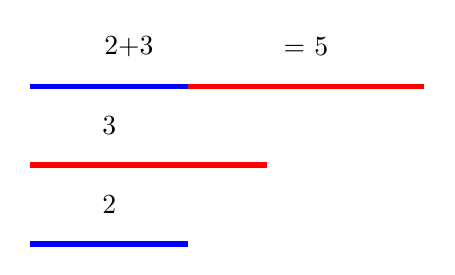
\begin{tikzpicture}

\draw[blue, line width=2 ] (0,2)--(2,2);
\draw[red , line width=2 ] (2,2)--(5,2);
\draw[red , line width=2 ] (0,1)--(3,1);
\draw[blue, line width=2 ] (0,0)--(2,0);

\node at (1,0.5) {2};
\node at (1,1.5) {3};
\node at (1.25 ,2.5) {2+3};
\node at (3.5,2.5) {= 5};

\end{tikzpicture} \\ \\
Tao - and Green, somewhat - have become suspect of the basic number operations.  $+$, $\times$, $-$, $\div$ if you do it too much and then someone tells you that it's wrong. So, let's try  new kind of number!

\newpage

\noindent \textbf{5/2} I would like to try to fill in the part about Galois cohomology.  Leading to the side issues like dynamics and computabiity, so the scenery is very rich.  \\ \\
We are trying to show that $x^2 = 2$ has no solutions in rational number $x \in \mathbb{Q}$ or (clearing denominators) $a^2 = 2b^2 $ has no solutions $a,b \in \mathbb{Z}$.  There seems to be a way using \textbf{heights} and a way using \textbf{torsors} but every book reviews it differently.  And hopefully we see what this cohomology nonsense is about. \\ \\

\vfill


\noindent Here's a reading list. I will leave in the Class Field Theory book since even though don't need it any way (we are solving over $\mathbb{Z}$), in fact we may need it anyway.

\begin{thebibliography}{}

%\item Nancy Childress \textbf{Class Field Theory} (Universitext).  Spinger, 2009.

\item Ben Green, Terence Tao, Tamar Ziegler. \textbf{An inverse theorem for the Gowers $U^{s+1}[N]$-norm} \texttt{arXiv:1009.3998}

\item Ben Green \textbf{Approximate algebraic structure} \texttt{arXiv:1404.0093}

\item W. T. Gowers \textbf{Generalizations of Fourier analysis, and how to apply them} \texttt{arXiv:1608.04127}

\end{thebibliography}

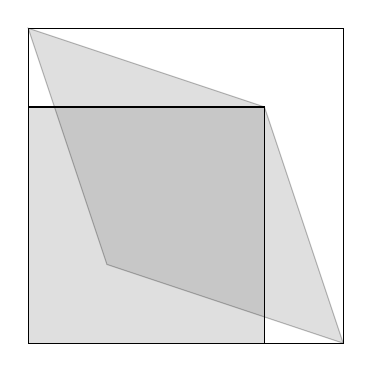
\begin{tikzpicture}
\draw (0,0)--(4,0)--(4,4)--(0,4)--cycle;
\draw[opacity=0.25, fill=black!50!white] (0,0)--(3,0)--(3,3)--(0,3)--cycle;
\draw (0,0)--(3,0)--(3,3)--(0,3)--cycle;
\draw[opacity=0.25, fill=black!50!white] (1,1)--(4,0)--(3,3)--(0,4)--cycle;
\draw (0,0)--(3,0)--(3,3)--(0,3)--cycle;
\end{tikzpicture}

\end{document}